%-*- coding: UTF-8 -*-
% 论文总结.tex
% 2020年7月第二周
\documentclass[UTF8]{ctexart}
\usepackage{graphicx}
\usepackage{float}
\usepackage{amsmath}
\usepackage{geometry}
\geometry{a4paper,centering,scale=0.8}
\usepackage[format=hang,font=small,textfont=it]{caption}
\usepackage[nottoc]{tocbibind}
\usepackage{url}
\usepackage{listings}
\usepackage{booktabs}
\usepackage{xcolor}     %高亮使用的颜色
\definecolor{commentcolor}{RGB}{85,139,78}
\definecolor{stringcolor}{RGB}{206,145,108}
\definecolor{keywordcolor}{RGB}{34,34,250}
\definecolor{backcolor}{RGB}{220,220,220}

\lstset{
 columns=fixed,       
 numbers=left,                                        % 在左侧显示行号
 numberstyle=\tiny\color{gray},                       % 设定行号格式
 frame=none,                                          % 不显示背景边框
 backgroundcolor=\color[RGB]{245,245,244},            % 设定背景颜色
 keywordstyle=\color[RGB]{40,40,255},                 % 设定关键字颜色
 numberstyle=\footnotesize\color{darkgray},           
 commentstyle=\it\color[RGB]{0,96,96},                % 设置代码注释的格式
 stringstyle=\rmfamily\slshape\color[RGB]{128,0,0},   % 设置字符串格式
 showstringspaces=false,                              % 不显示字符串中的空格
 language=c++,                                        % 设置语言
}

\newenvironment{myquote}
{\begin{quote}\kaishu\zihao{-5}}
{\end{quote}}

\newcommand\degree{^\circ}

\title{\heiti A Framework for Quantitative Security Analysis of Machine Learning}
\author{\kaishu 宇翔}
\date{\today}

\bibliographystyle{plain}

\newtheorem{thm}{定理}

\begin{document}
    
    \maketitle

    \clearpage
    \section{摘要}\label{sec:diyijie}
	本文提出了一种用于定量分析机器学习方法安全性的框架。该框架的关键问题是部署学习模型和攻击者约束的形式规范,最佳攻击行为的计算以及推导机器学习算法对抗性影响的上限。理解机器学习算法安全性的关键在于根据攻击者的目标和应用程序的特定限制对其进行定量分析。本文提出的学习方法安全性分析框架定义了此类分析中要解决的关键问题,文章示范了如何将该框架应用于一种特定学习场景(在线质心异常检测?),分析其安全性。本文提出该框架希望能有助于开发强大的对抗性学习方法。
	\clearpage

    \section{本文所提出的框架}\label{sec:dierjie}
	本文提出的框架是针对机器学习的攻击不考虑最坏情况下(即攻击者可以任意操纵数据),开展一种“合理情况”的分析。即在合理假设下,攻击者能否获得可用的攻击,攻击能否成功。这些假设可能因应用程序而异。因此,必须明确说明这些条件,并且分析必须解决攻击有效性与攻击者的约束和资源消耗之间的相互依赖性。为了解决这些问题,提出了以下四步过程来对机器学习方法进行安全性分析。
	\begin{itemize}
	\item[1] 公式化攻击过程和学习过程。(需说明攻击者能够利用的知识以及其攻击目标)。
	[\begin{upshape} \itshape Axiomatic formalization of the learning and attack processes. The first step in the analysis is to formally specify the learning and attack processes. Such formalization should include definitions of data sources and objective (risk) functions used by each party. It should specify the knowledge available to an attacker,i.e. whether he knows an algorithm, its parameters and internal state, and which data he can potentially manipulate. Finally, the attack goal should be also specified. \end{upshape}]
	\item[2] 指定攻击者的约束条件(攻击者方面的潜在限制可能包括:受其控制的流量百分比,要注入的其他数据量等)
	[\begin{upshape} \itshape Specification of attacker’s constraints. Potential constraints on the attacker’s part may include: percentage
	of traffic under his control, amount of additional data to be injected, an upper bound on the norm of manipulated part, a maximal allowable false-positive rate (in case an attack must stealthy), etc. Such constraints must be incorporated into the axiomatic formalization.\end{upshape}]
	\item[3] 研究最佳攻击策略
	[\begin{upshape} Investigation of an optimal attack policy. Given a formal description of the problem and constraints, an optimal attack policy must be investigated. Such policy may be long-term, i.e. over multiple attack iteration,as well as short-term, for a single iteration. Investigation can be carried out either as a formal proof or numerically, by casting the search for an attack policy as an optimization problem. \itshape \end{upshape}]
	\item[4] 分析最佳攻击策略下攻击者的收益界限。例如计算攻击成功率,估算攻击迭代次数等。
	[\begin{upshape} \itshape  Bounding of attacker’s gain under an optimal policy. Finally, the progress of an attack towards its goal under an optimal policy must be analyzed. Such analysis may take different forms, for example calculation of the probability for an attack to succeed, estimation of the required number of attack iterations, calculation of the geometric impact of an attack (a shift towards an insecure state), etc.\end{upshape}]
	\end{itemize}
	对机器学习安全性的研究必须考虑以下两个方面:
	\begin{itemize}
		\item[1] 对攻击者破坏学习过程所需资源进行定量分析
		\item[2] 分析师必须考虑到攻击者存在的约束条件
	\end{itemize}
	文章提出的框架有两方面的意义:1、使人们能够在相同条件下定量分析和比较现有算法。2、使研究者在机器学习方面从安全性,准确性和资源消耗之间进行权衡分析。按照统计学的理论,需要紧凑的模型来实现高学习精度。但是,此类模型可能更容易被攻击者破坏。通过提供安全风险的定量度量,本文提出的框架可用于设计学习算法的最佳风险函数。
	\clearpage

	\section{在线质心异常检测的定量分析}\label{sec:disnajie}
	在线异常检测可能是中毒攻击(是不是这么翻译)的对象,其目标是迫使算法接受位于正常范围之外的攻击向量。文章通过对攻击者攻击场景的建模,评估算法的安全性:攻击行为是否成功很大程度上取决于攻击者控制的训练数据的比例。当小于临界值时,攻击进度受常数限制,这也就意味着即使攻击者能够进行无条件限制攻击也无法成功。(示例不是特别理解,mark一下先)
	\begin{figure}[ht]
        \centering
        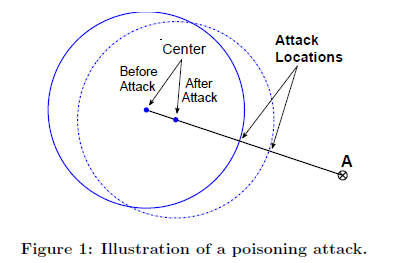
\includegraphics[scale=0.8]{picture/001.png}
        \caption{质点变化中毒攻击}
        \label{fig:001}
    \end{figure}
    \begin{figure}[ht]
        \centering
        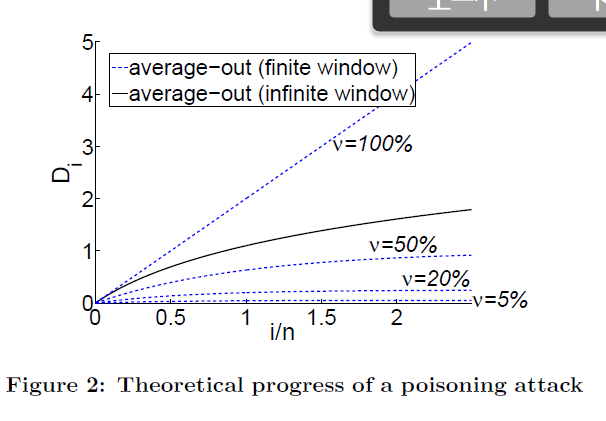
\includegraphics[scale=0.8]{picture/002.png}
        \caption{中毒攻击理论过程}
        \label{fig:002}
    \end{figure}
	\clearpage
	\section{案例}\label{sec:disijie}
	本部分介绍了如何在实践中应用该分析:针对监视HTTP流量的质心异常检测器模拟了一次中毒攻击。 每个入站HTTP请求的有效负载都被视为单个数据点,创建良性数据集和恶意数据集,根据攻击者能够获取到的先验知识(可以在网络上进行嗅探),构建攻击场景(攻击者可以计算法线数据质心的位置并生成要注入的点),通过实验验证(2950个良性数据点的质心,并计算质心和攻击矢量之间的相对位移D,如果观察到的相对位移达到0.179的临界值,则攻击成功),计算出攻击者必须控制至少15%的数据才能使攻击成功。
	\clearpage
	\section{摘要}\label{sec:diwujie}
	本文提出了一种用于定量分析机器学习方法安全性的框架。该框架的关键问题是部署学习模型和攻击者约束的形式规范,最佳攻击行为的计算以及推导机器学习算法对抗性影响的上限。理解机器学习算法安全性的关键在于根据攻击者的目标和应用程序的特定限制对其进行定量分析。本文提出的学习方法安全性分析框架定义了此类分析中要解决的关键问题,文章示范了如何将该框架应用于一种特定学习场景(在线质心异常检测?),分析其安全性。本文提出该框架希望能有助于开发强大的对抗性学习方法。
	\clearpage
	\section{补充}\label{sec:diliujie}
	\subsection{马氏距离}
	试考虑一个数据点是否属于某一分布的概率问题。第一个步骤是找到质心或者说样本点的质量中心。直观上来看,该点离质心越近,越可能属于这个集合。然而,我们也要注意该集合的范围大小,这样我们才能判断给定的离质心的距离是否值得注意。简化的方法是去估计样本点与质心距离的标准差。将其插入标准分布中,我们可以得出数据点是否属于同一分布的概率值。
	
	上述方法也存在缺陷,我们假设了样本点相对于质心是球形分布的。如果它们的分布不是球状的,而是椭圆状的,我们在判断测试点是否属于该集合时,不仅要考虑与质心的距离,还要考虑方向。在那些椭圆短轴的方向上,测试点的距离一定更近,但那些长轴方向上测试点是远离质心的。从数学角度看,我们可以通过计算样本的协方差矩阵,来估计出最能代表集合分布的椭圆。马氏分布是指从测试点到质心的距离除以椭圆在测试点方向上的宽度。

	为了使用马氏距离来判别一个测试点属于 N 个分类中的哪一个,首先应该基于已知样本与各个分类的对应情况,来估计每个类的协方差矩阵。在我们的例子中,我们只对“正常”和“异常”两个类别感兴趣,我们使用只包含正常操作状态的数据作为训练数据,来计算协方差矩阵。接下来,拿来测试样本,计算出它们与“正常”类别的马氏距离,如果距离高于所设置的阈值,则说明该测试点为“异常”。 

	\subsection{中毒攻击}
	最为常见的中毒攻击就是DNS缓存的中毒攻击。具体做法就是污染DNS缓存,使得用户访问错误的网站。
	使用机器学习的方法建立异常检测模型的时候,如果攻击者去污染建立模型的数据,就会使得模型建立出现偏差。如果攻击者有目的性的去设置样本,用以干扰质心的位置,那么整个异常检测的模型便是不可靠的。
	\clearpage
	\bibliography{test}
\end{document}

